\documentclass[letterpaper]{article}
\usepackage[T1]{fontenc}
\usepackage[pdfusetitle,colorlinks]{hyperref}
\usepackage[pdftex]{graphicx}
\usepackage{verbatim}
\usepackage{amsmath}
\usepackage{booktabs}
\usepackage[font=scriptsize,labelfont=bf,margin=3em]{caption}

\newcommand{\cpp}{C{\nobreak+}{\nobreak+}}

\newcommand{\code}[1]{\small\textsf{#1}}

\renewcommand{\_}{\allowbreak\textunderscore\allowbreak}


\title{Genetic Chess}
\author{Mark Harrison}

\begin{document}

\maketitle

\begin{abstract}
This work is a program for evolving chess-playing AIs.  By pitting a population of AIs against each other in chess matches, killing off the losers, and breeding the winners, it is hoped that one specimen will be able to stand up against a more traditionally developed engine (if only on the easiest difficulty setting). Though it is written in \cpp{}, it is the hope of the author that the style and architecture are comprehensible.
\end{abstract}

\tableofcontents{}


\section{Building}
There is nothing OS-specific about the \cpp{} code, so the code can be compiled with any \cpp{} compiler via
\begin{quote}
	\code{<compiler> -I include -D NDEBUG <all *.cpp files>}
\end{quote}
where \code{-I} indicates the option to specify the base directory of the header files and \code{-D NDEBUG} instructs the compiler to skip tests and assertions. For testing and debugging, use
\begin{quote}
	\code{<compiler> -I include -D DEBUG <all *.cpp files>}
\end{quote}
instead.

\subsection{Linux}
Run \code{make} to create various executables in a \code{bin/} subfolder that will be created if it does not already exist. If, in the course of working on this project, new files are created or the \code{\#include} files are changed within a file, run \code{python create\_Makefile.py [compiler]} to regenerate the Makefile. The choices for the compiler are \code{gcc} and \code{clang}. These python script assumes all \code{*.cpp} files in the current directory and all subfolders are part of the project and need compiling. Then, run \code{make} to build any of the following: \code{build} for an executable with debugging symbols and no optimization, \code{profile} for an optimized build that generates profiling information while running, and \code{release} for a fully optimized executable.

\subsection{Windows}
The \code{.sln} and \code{.vcxproj} files are project files for Visual Studio. These will load all source files for one-click compiling.


\section{Running}\label{running}
\begin{description}
	\item[\code{genetic\_chess -test}] Run tests of the program for chess rule conformance and for Genetic AIs working properly.
	\item[\code{genetic\_chess -genepool [file name]}]
This will start up a gene pool with Genetic\_AIs playing against each other---mating, killing, mutating, all that good Darwinian stuff. The required file name parameter will cause the program to load a gene pool and other settings from a configuration file. A record of every genome and game played will be written to text files.

	\item[\code{genetic\_chess <-player> <-player>}] Starts a local game played in the terminal with an ASCII art board. The first parameter is the white player, the second is black. The \code{<-player>} argument is replaced with one of the following:
	\begin{description}
		\item[\code{-human}:] a human player entering moves on the command line and seeing the results on a text-based drawing of the board. Moves are specified in standard algebraic notation (SAN) or in coordinates that indicate the starting and ending square.
		\item[\code{-genetic [file name [number]]}:] a Genetic AI player. If a file name follows, load the genes from that file. If there are several genomes in a file, the file name can be followed by a number to load the genome with that ID\@. If no number is specified, then there are two possibilities:
		\begin{itemize}
			\item If the genome file is the output of a gene pool run, then the AI with the smallest ID that was still alive is chosen. As the oldest surviving AI, it is the nearly the most evolved while still having been tested.
			\item Otherwise, the last genome in the file is loaded (presumably this one is the most evolved). If there is another file containing records of games played during a gene pool run that has the same name as the genome file name with an extra suffix ``\_games.txt'', then the last genome with at least 3 wins will be selected.
		\end{itemize}
		\item[\code{-random}:] an AI player that chooses a random legal move at each turn.
		\item[\code{-turing}:] a chess engine implemented according to the design by Alan Turing~\cite{turing-chess}.
		\item[\code{-montecarlo}:] a chess AI that picks a move based on the results of randomly played complete games, i.e., the pure version of Monte Carlo tree search~\cite{monte-carlo}. A warning: this AI can be very memory intensive depending upon the computer's speed and the time controls of the game. On my computer, 5/40 time control results in almost 900~MB of memory usage per player.
	\end{description}
\end{description}
Genetic Chess can communicate with GUI chess programs through the \href{https://www.gnu.org/software/xboard/engine-intf.html}{Chess Engine Communication Protocol}, including xboard, PyChess, Cute Chess, and others. When using Genetic Chess this way, only specify the arguments for a single player (\code{-genetic} or \code{-random}). The program will then wait for communication from the GUI\@.


\section{Non-Evolutionary Aspects}

These sections describe the aspects of the chess AI that are not genetically modifiable, usually because of at least one of the following reasons:
\begin{itemize}
	\item There is no sense in which the aspect of play is improvable. Any modification would be detrimental to the chess playing;
	\item It would take far too much time to evolve that aspect of play from a random starting configuration, or it would interfere too much with the evolution of other aspects;
	\item I cannot conceive of how to represent the state space of that particular play strategy so that it may be genetically encoded.
\end{itemize}
On the last point, it has been suggested to me that, instead of the specific genes listed in Section~\ref{gene-section}, the genes should encode more abstract and generic strategies and heuristics for evaluating a board state. While this would probably better mimic biological evolution (wherein adenine and thymine are rather neutral as to their teleology), I have no idea how to program such an abstract representation and how to translate the action of such genes into chess moves. So, what results from all this programming is a glorified tuning algorithm for parameters in predefined genes with hard-coded meanings.

On the other hand, so is every other genetic algorithm (see~\cite{evolved-antenna},~\cite{evolved-stellarator}, and others). Plus, these genes can evolve to have near-zero influence on game decisions, so these AIs are perfectly capable of telling me exactly what they think of my painstakingly crafted genes.\footnote{The little ingrates!}

\subsection{Endgame Scoring}

Winning gives a positive infinite score.
Losing gives a negative infinite score.
Draw gives zero.

Why not evolve these numbers? While the priorities of various genes can be varied to yield different playing styles, the only reasonable score to assign to a win is one that is larger than any other score. It can only be a disadvantage to prefer anything to a winning move. While this would result in upward evolutionary pressure on the score assigned to winning, it would stall the evolution of all other genes while the score assigned to winning was pushed high enough to always be preferred.

The specific values were chosen to make the scoring symmetrical between the two players, in that the score for one side is the negative of the score as seen from the other side (assuming the same player does the scoring). What is good for one player is bad for the other player by the same amount.

\subsection{Mini-maxing}

The principle behind the minimax algorithm is that the quality of a move is measured by the quality of moves it allows the opponent to make. Of course, the quality of those moves is measured by the quality of the moves that follow. Ideally, the only required board evaluation scores would be \(1\)~for a win, \(0\)~for a draw, and \(-1\)~for a loss, and all possible sequences of moves would be examined to find the guaranteed outcome. Unfortunately, the number of positions to examine in a typical game is far too large to examine in a few minutes, so the search has to be cut off at some point and a heuristic evaluation employed to estimate the probability of winning from that stopping point. In this program, the decision of when to stop and the heuristic evaluation is genetically determined and evolved over many generations.

\subsection{Alpha-Beta Pruning}

Alpha-beta pruning is based upon keeping a record of two game state evaluations:
\begin{description}
	\item[Alpha:] is the highest guaranteed score that the player whose turn it is can reach once the game reaches the current state (i.e., the root of the current game tree) and cannot be avoided by the opponent making different moves later in the game. That is, the player whose turn it is at this point in the game tree can force the game into a state with at least this score.
	\item[Beta:] is the lowest score to which the opponent can limit the current player by making moves that avoid higher scores. If the current player finds a move with a higher score than Beta, then the opponent would make a different move earlier in the game that makes this game state impossible to reach. This earlier move is called a ``refuting'' move. Once a move is found that is refuted by an earlier opponent move, the examination of that set of moves is abandoned, as the opponent will not allow the game to reach that state.
\end{description}
Each time a move examination reaches a greater depth in the game tree, these values switch roles to represent the view of the board from the opponent's perspective.

An extra optimization implemented in this program is one where the search is cut off if Alpha represents a win at a shallower depth in another branch of the tree branch. If a checkmate can be forced in fewer moves by making different earlier moves, there's no point in looking for a win in the current move sequence.

\subsection{Principal Variation Recall}

If the best move is chosen based upon the probable resulting future board state based on a sequence of moves (a variation) found through minimaxing with alpha-beta pruning, and if the opponent makes the next predicted move in that variation, then the moves leading to that board state are examined first during the next move. This high-scoring board state should lead to early cutoffs from alpha-beta pruning, especially if that board state was a game-ending state. If that board state is actually avoidable by the opponent, then the shallower depth of that state during the next turn should lead to a faster refutation, leaving time to examine alternate variations.

\subsection{Move Ordering}

Besides Principal Variation Recall, those moves that capture an opponent's piece are examined before other moves. Capturing moves usually result in the largest changes in position evaluations (see Section~\ref{total-force-and-pawn-result}), so they should quickly establish alpha and beta values that will lead to quick cutoffs.

\section{The Genome}\label{gene-section}
The genome is the repository for genetic information in the Genetic AIs and controls all aspects of game play not mentioned in the previous section. All are subject to mutation, which can change the behavior and influence of a given gene.

\subsection{A Note on Designer Genes}

Evolution is an effective means of optimizing when every mutation makes a difference in the fitness of an organism. In an abstract sense, the fitness function of an organism should be
\begin{enumerate}
	\item a continuous function of the parameters of its genome and
	\item without flat sections.
\end{enumerate}
The first of these qualities is due to the fact that large changes in behavior are rarely beneficial. A small change to the genome should not result in a large change in behavior. This is why the deactivating-gene mutation was discarded. It is better to let a gene fall in importance by gradually reducing its priority. The second point means that gene parameters should not be allowed to take on values where mutations no longer have any affect on behavior. This leads to random walk types of gene movements until the gene parameters once again reached a range of values that changed the behavior of the AI\@. This random walk period only represents wasted time. To this end, certain gene parameters are restricted to, for example, non-negative values.

\subsection{Regulatory Genes}
A regulator gene refers to a gene that does not participate in evaluating the state of a game board. These genes either control other aspects of the Genetic AIs or are queried by other genes for information.

\subsubsection{Piece Strength Gene}\label{piece-strength}

This gene specifies the importance or strength of each different type of chess piece. Other genes like the Total Force Gene (Section~\ref{total-force}) reference this one for their own evaluation purposes.

Previously, the king was not assigned a strength because it is always on the board, so it cannot affect the move chosen. This is not quite true. The score returned by the Total Force Gene cannot be affected by the king's strength because there is always one black and one white king on the board, canceling their contribution to a board position's score (see Sections~\ref{board-score-section} and~\ref{total-force}). However, the Opponent Pieces Targeted Gene does have a use for that value, since putting an opponent in check is an important component of the game. Some surprising results of adding a strength value for the king are discussed in Section~\ref{piece-strength-with-king}.

\subsubsection{Look Ahead Gene}
This gene determines all aspects of the Genetic AIs time management through a set of genetically determined components to this gene that determine how the AI spends its time:
\begin{enumerate}
	\item the average number of moves per game,
	\item the uncertainty in the above average.
	\item a constant related to over-allocating search time while counting on alpha-beta pruning to not use too much
\end{enumerate}
When the AI starts the algorithm to choose a move, it allocates a fraction of the time left on the clock so that all subsequent moves get equal time. That is, if there are 20~moves estimated to be left in the game, then \(1/20\)~of the remaining time is used for this move. The number of moves left is estimated by assuming the number of moves in a game is modeled by a log-normal distribution~\cite{log-norm-wiki}\cite{log-norm-chess-se} with a mean and spread given by the first two parameters listed above. Originally, it was assumed that the number of moves in a game was well-modeled by a Poisson distribution. This proved to be false (see Figure~\ref{game-length-plot}), and the log-normal distribution---wherein the logarithm of the variable is normally distributed---is now used.

The number of moves left in the game is estimated by
\[N(n) = \frac{\sum_{i = n + 1}^\infty P(i)\times{}i}{\sum_{i = n + 1}^\infty P(i)} - n\]
where \(N(n)\) is the estimated number of moves left in the game given that \(n\) moves have already been made, and \(P(i)\) is the \emph{a priori} probability distribution of the number of moves by one player in a single game. The numerator is a truncated calculation of the average number of moves in a game, and the denominator is a truncated probability distribution to renormalize (since the probability of a game lasting 10~moves is zero if 11~moves have been played).

The log-normal probability distribution is given by
\[P(x) = \frac{1}{xS\sqrt{2\pi}} e^{-\frac{1}{2}{\left(\frac{\ln{x} - M}{S}\right)}^2},\]
where \(S\) and \(M\) are the standard deviation and mean of the logarithm of the number of moves in a game, respectively. Even though this is a continuous probability distribution, it is a good fit for the length of chess games as can be seen in the plot of the number of moves in a long gene pool run can be seen in Figure~\ref{log-norm-plot}. Instead of using the summation formula above to estimate the number of moves remaining in the game, the result can be approximated with integrals\footnote{Courtesy of Wolfram Alpha: \url{http://www.wolframalpha.com/}} to yield a closed-form expression using function available in native \cpp.
\begin{align*}
\sum_{i = n + 1}^\infty P(i)\times{}i &\approx \int_{n+1}^\infty P(t)t dt \\
	&= \frac{1}{S\sqrt{2\pi}} \int_{n+1}^\infty e^{-\frac{1}{2}{\left(\frac{\ln{t} - M}{S}\right)}^2}dt\\
	&= \frac{1}{2}e^{M + S^2/2}{\left[1 + \textrm{erf}{\left(\frac{M + S^2 - \ln n}{S\sqrt{2}}\right)}\right]}
\end{align*}
and
\begin{align*}
\sum_{i = n + 1}^\infty P(i) &\approx \int_{n+1}^\infty P(t)dt \\
	&= \frac{1}{S\sqrt{2\pi}} \int_{n+1}^\infty \frac{1}{t} e^{-\frac{1}{2}{\left(\frac{\ln{t} - M}{S}\right)}^2}dt \\
	&= \frac{1}{2}\left[1 + \textrm{erf}\left(\frac{M-\ln n}{S\sqrt{2}}\right)\right].
\end{align*}
Here, \(\textrm{erf}\) is the error function given by
\[
\textrm{erf}(x) = \frac{2}{\sqrt{\pi}}\int_0^x e^{-t^2}dt
\]
This results in the number of moves left in a game (\(N(n)\)) after \(n\) moves is
\[
N(n) = \left(e^{M + S^2/2}\right) \frac
{1 + \textrm{erf}\left(\frac{M + S^2 - \ln n}{S\sqrt{2}}\right)}
{1 + \textrm{erf}\left(\frac{M-\ln n}{S\sqrt{2}}\right)}
- n.
\]
\begin{figure}[tbh]
	\centering
	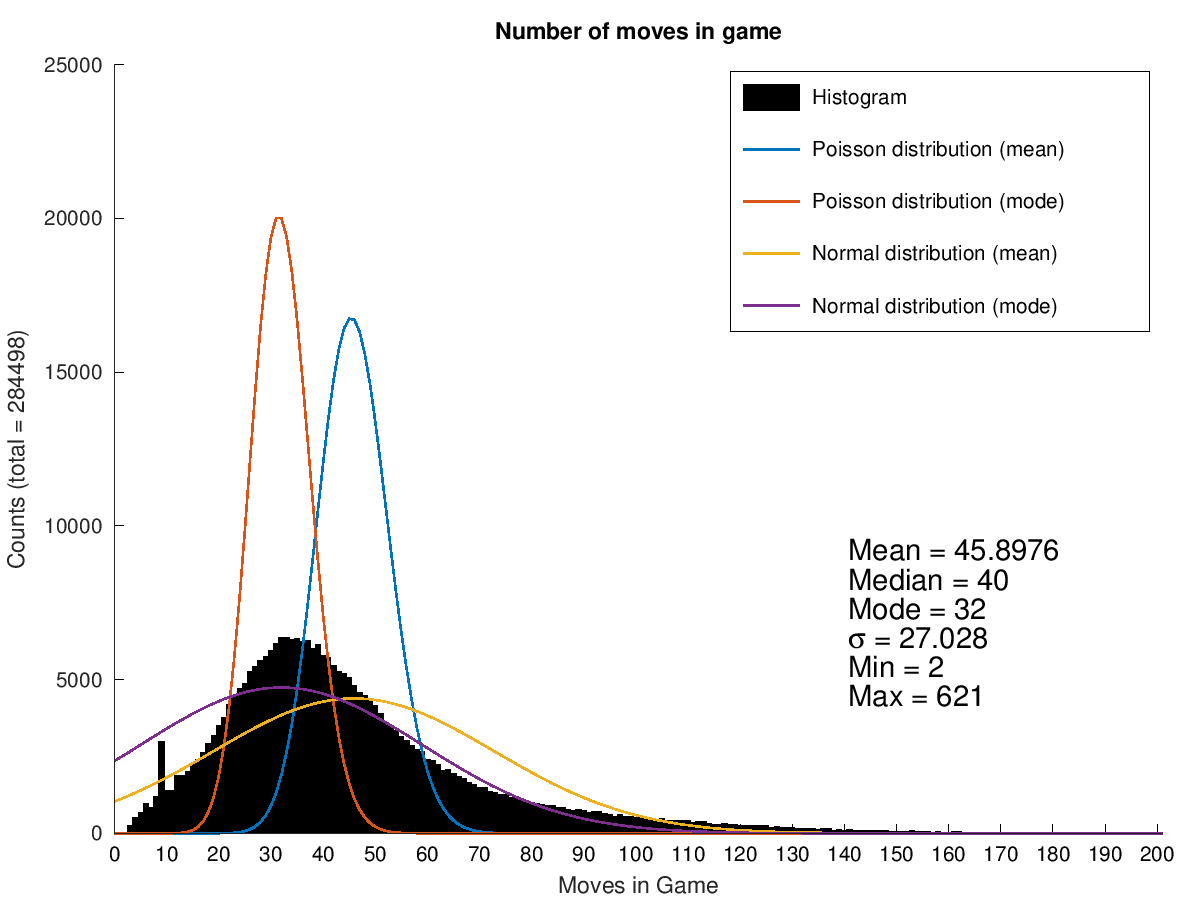
\includegraphics[width=0.7\textwidth]{game_length_distribution.png}
	\caption{First attempts at determining the distribution of moves in chess games. The black histogram shows the distribution of the number of moves in a game (with one move consisting of both a black and white play). The (mean) and (mode) designations in the legend indicate which statistic was used as the mean parameter of the fitted Poisson and normal distributions (neither of which are a good fit). The spike at 9~moves was created just after a change to the program that resulted in much faster changes in board state.}\label{game-length-plot}
\end{figure}

\begin{figure}[tbh]
	\centering
	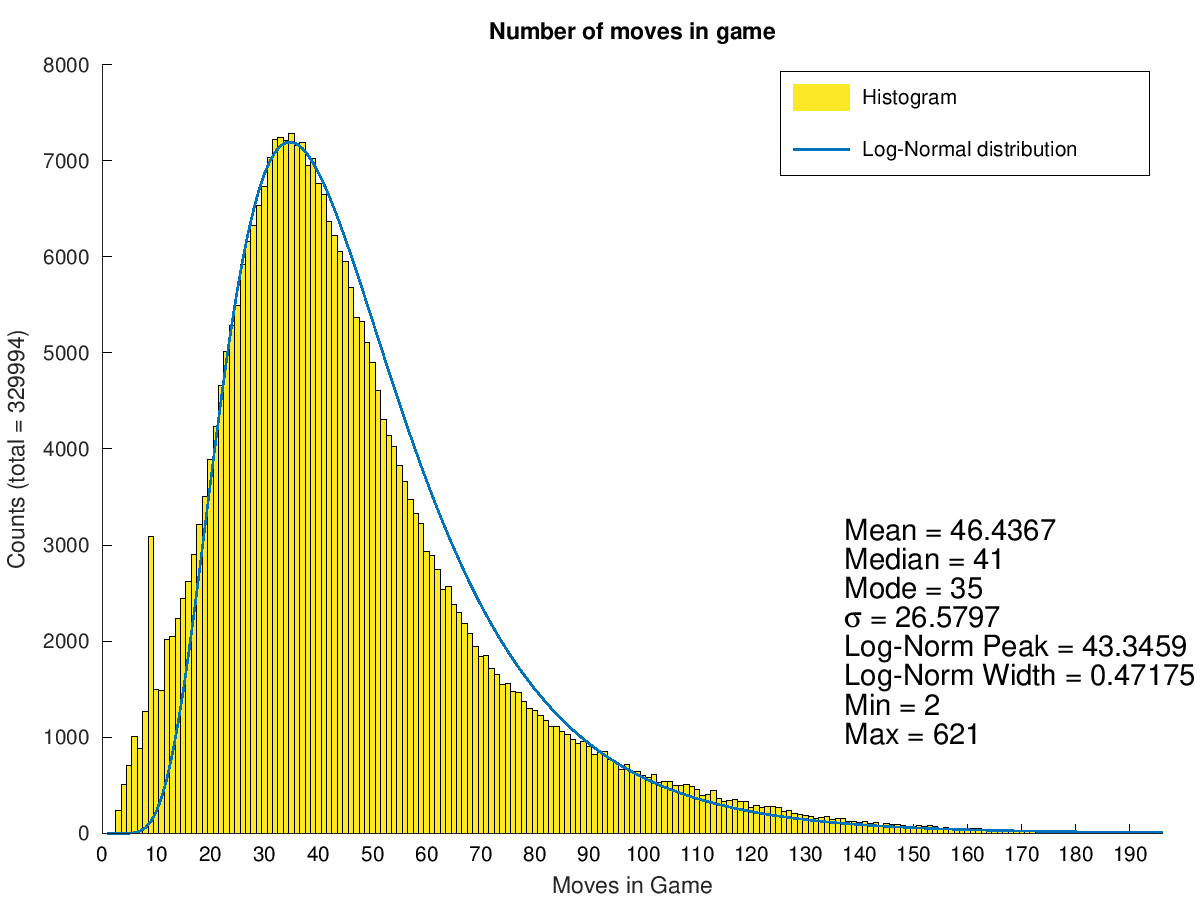
\includegraphics[width=0.7\textwidth]{game_length_log_norm_distribution.png}
	\caption{The distribution of the number of moves in a game with a log-normal fit. The Log-Norm parameters listed are \(M\) for the Peak parameter and \(S\) for the Width parameter. To obtain a better fit, only games longer than 15~moves were considered, as shorter games were primarily by ill-adapted AIs (especially the spike at 9-move games), especially at the beginning of the gene pool run.}\label{log-norm-plot}
\end{figure}

If the number of moves left in the game is greater than the number of moves that will result in a clock reset, then the latter will determine how much time will be used. In a game with 40/5~time control, where five minutes are added to the clock every 40~moves, every 40th move can use all the remaining time since an extra five minutes will be added after the move. Whatever the final number of moves left is used, the time on the clock is divided by that number to determine how much time to take to choose a move.

When choosing a move from the current board, the amount of time to consider a move is equal to the amount of time left for this board position divided by the number of legal moves left to consider. This naturally limits the depth of search while allowing deeper searches for positions with fewer legal moves, which are often a series of forced moves due to check and so deserve deeper inspection. If a move examination is cut off early for whatever reason (e.g., a game-ending move is found or through alpha-beta pruning), then the remaining time is available for as yet unexamined moves.

An effective chess player needs to look at the consequences of a move to decide if a move is good. In order to decide how far to look ahead (and if there is time remaining to examine this move), at each step, the AI divides the number of legal moves in the board position after the move under consideration by the number of positions it can examine per second.
\[
T = k\frac{N_{\textrm{legal}}}{v}
\]
where \(T\) is the time needed to look ahead on this move, \(N_{\textrm{legal}}\) is the number of legal moves on the board after the move is made, \(v\) is the rate of position examinations, and \(k\) is a genetically determined speculation constant that adjusts the amount of time to use. The speed \(v\) is determined by counting the number of positions evaluated (leaf nodes in the game tree) and dividing by the amount of time spent evaluating during the previous move. If the time \(T\) is less than the time allocated for the move, the algorithm looks ahead (the search function recurses) to examine the moves the opponent can make in response. Otherwise, it evaluates the current position and moves on to the next legal move.

The speculation constant has four possible values depending on whether
\begin{enumerate}
	\item the move under consideration captures or promotes (Just Changed Material),
	\item the board position after the move has a capturing or promoting move (Can Change Material),
	\item both of the above are true (Material Exchange),
	\item none of the above are true (Default).
\end{enumerate}
The names in parentheses are the labels used in the source code and genome analysis plots. These board qualities were chosen since material changes can very rapidly change the evaluation of boards, requiring further examination until the board reaches a less volatile state. Capturing a piece or promoting a pawn is only good if it doesn't result in a greater loss in subsequent moves. This is the problem that is usually solved in other chess engines by a quiescence search, in which all interesting\footnote{Meaning, captures that aren't immediately losing.} capturing moves are performed on a board before it is scored, thereby only scoring stable, ``quiescent'' board states~\cite{quiescence-ref}.

\subsubsection{Mutation Rate Gene}\label{mutation-rate-gene}
This gene controls how many randomly chosen genes get mutated every time there's a call to \code{Genome::mutate()}. The unique aspect of this gene is that it is the only one that does not change the behavior of the AI during its lifespan. Mutations only occur upon birth, so this gene only controls how the offspring of the containing AI are modified. There is a risk that a moderately successful AI will shutdown mutation to preserve a currently winning genome. Thus, the minimum number of mutations is one.

\subsection{Board-Scoring Genes}\label{board-score-section}

These genes are used to give a score to a board state. The higher the score, the more desirable the moves that lead to this board. The score is calculated by
\[Score = \sum_g Priority(g) \times Score(g,B)\]
where \(g\) represents each gene, \(Priority(g)\) is a genetically determined scalar multiplicative factor that determines how much the gene's score of the board influences the final score, and \(Score(g,B)\) is the result of the scoring procedure of that gene on a given board \(B\).

Since it is not only important to find position that are advantageous to the player, but also disadvantageous to the opponent, the final heuristic score for a board position is given by
\[Heuristic\ Score = Score(Player) - Score(Opponent).\]

In general, the scoring function outputs of each gene are scaled so that a typical board state gets a score near one. For example, the Freedom to Move Gene divides the number of legal moves by the number of legal moves at the start of the game (20 for standard chess). This way, the priorities of genes can be easily compared as evolution progresses.

Some of the board-scoring genes are forced to have non-negative priorities as a way of speeding up the optimization. As an example, the Total Force Gene (Section~\ref{total-force}) has a non-negative priority because its scoring method relies on values from the Piece Strength Gene (Section~\ref{piece-strength}). The score returned is basically the product of the priority of the Total Force Gene and the values of the piece strengths. When both of these are allowed to mutate to both positive and negative values, they often get stuck near zero. When one changes sign, the other is driven towards changing sign as well to get back to better evaluation results. Forcing the priority to be positive puts a consistent pressure on the piece strengths to get to their proper values (whether positive or negative). This does not limit the behavior of the Genetic AIs since the piece strengths could evolve to negative strengths if the AI wants to lose its pieces.

\subsubsection{Total Force Gene}\label{total-force}
This gene sums the strength (according to the Piece Strength Gene) of all the player's pieces on the board except the king. The king is left out for two reasons. First, there is always a black king and a white king on the board, so they cancel. Second, this exception leaves the king value to be determined by the Opponent Pieces Targeted Gene (Section~\ref{opponent-pieces-targeted}), essentially determining the value of putting the other player in check. The score returned is divided by the total value of the starting set of pieces (8~pawns, 2~rooks, 2~knights, 2~bishops, and 1~queen) so that the result is between~0 and~1.

As noted in Section~\ref{board-score-section} above, the priority of this gene is restricted to be non-negative.

\subsubsection{Freedom to Move Gene}
This gene counts the number of squares under attack by a side that are also not occupied by friendly pieces. This represents how many moves are available without considering whether the king is in check or if any pieces are pinned. This count is divided by the number of squares under attack at the beginning of a game to bring the maximum score near one.

\subsubsection{Pawn Advancement Gene}
This gene measures the progress of all pawns towards the opposite side of the board. The gene includes a non-linearity term that controls how the position of the moving pawn affects the score as it moves.
\[S = \frac{1}{8}\sum_p \left|\frac{rank(p) - home(p)}{5}\right|^{1 + N}\]
Here, \(S\) is the total score, the sum is over all pawns \(p\) of the scoring side, \(rank(p)\) is the rank position of the current pawn, \(home(p)\) is the home rank of the pawn (2~for White and~7~for Black), and \(N\) is the non-linear term. A positive \(N\) means more points are awarded as the pawn advances farther from the home rank. A negative \(N\) rewards moving pawns off the home rank. The division by~5 (the farthest a pawn can advance before promotion) and the division by~8 (the maximum number of pawns) normalize the score to be between~0 and~1.

\subsubsection{Passed Pawn Gene}
The gene counts the number of pawns that cannot be stopped or captured by an opponent's pawns. That is, a pawn is a passed pawn if there are no pawns ahead of it in its file or any directly adjacent files. Partial points are awarded for pawns that have fewer pawns ahead than usual (\(1/3\) for each free column ahead of mid-board pawns, \(1/2\) for for pawns on the edge).

\subsubsection{Opponent Pieces Targeted Gene}\label{opponent-pieces-targeted}
This gene sums the total strength (as determined by the Piece Strength Gene) of the opponent's pieces currently under attack. The returned result is divided by the total score of pieces at the start of the game, similarly to the Total Force Gene, although the value of the king is included in this divisor. Despite relying on values from the Piece Strength Gene, it is not restricted to non-negative priorities like the Total Force Gene because the Total Force Gene provides enough evolutionary pressure on the Piece Strength Gene to force it to a consistent sign.

Interestingly, since both kings are always on the board, they always cancel each others effect in the Total Force Gene, leaving this gene alone to drive their strength value. The result of this is discussed in the results section (Section~\ref{piece-strength-with-king}).

\subsubsection{Sphere of Influence Gene}
This gene counts the number of squares attacked by all pieces. Bonus points are awarded if the square can be attacked with a legal move. That is, if a piece cannot reach a square in one move (perhaps because such a move is blocked by another piece), then that square is still counted as falling under the influence of the side owning that piece. Further bonus points are awarded based on how close the attacked square is to the king. Because of its subcomponents, this gene's priority is restricted to non-negative values.

The effective formula for the score of this gene can be expressed as
\[score = \sum_s legal(s)\left(1+\frac{KTF}{1+distance(s,king)}\right)\]
where the sum is over all squares \(s\) on the board. The function \(legal(s)\) returns~0 if \(s\) is not attacked at all, or one of two genetically determined factors depending on if the the attack is legal (ignoring checks or pins) or not. An illegal move is one that is blocked by another piece. The term \(KTF\) is the king target factor and is a genetically determined weight that adjusts the importance of attacking squares close to the opposing king. The function \(distance(s_1, s_2)\) gives the distance between two squares in king moves and is equal to the maximum of the difference in file or rank between the squares. In the formula above, \(king\) represents the square the opposing king occupies.

\subsubsection{King Confinement Gene}
This gene tracks the manner in which the king is prevented from moving. In general, a king is safe if it is surrounded by friendly pieces or, failing that, it is free to move around the board when there are opposing pieces near. In scoring a board, this gene tracks the squares the king can reach given unlimited consecutive legal moves up to a genetically determined maximum distance.

For a more detailed picture, each square potentially reachable by the king is classified into three types given one of three genetically determined scores for each:
\begin{itemize}
	\item Free: the king is free to move on to these squares,
	\item Friendly block: the king is blocked by pieces of the same color, and
	\item Opponent block: the king is blocked due to the square being attacked by an opponent piece.
\end{itemize}
Note that opponent pieces by themselves do not block the king since they can be captured. Once all reachable squares have been found within a genetically determined maximum distance (measured in king moves), the score is calculated by the following:
\[S = \frac{W_{friendly}\sum_{s \in R}Friend(s) + W_{opponent}\sum_{s \in R}Opponent(s)}{\left(\left|W_{friendly}\right| + \left|W_{opponent}\right|\right)\left(1 + \sum_{s \in R}Free(s)\right)}
\]
where \(S\) is the resulting score, \(\sum_{s \in R}\) is a sum over every square \(s\) on the board that is reachable (\(\in R\)) from the current king location, \(W_{friend}\) is the genetically determined weight of squares blocked by friendly pieces, \(W_{opponent}\) is the genetically determined weight of squares blocked by opponent attacks, \(Friend(s)\) returns 1 if the square \(s\) is blocked by a friendly piece and 0 otherwise, \(Opponent(s)\) returns 1 if the square \(s\) is attacked by an opposing piece and 0 otherwise, and \(Free(s)\) returns 1 if the square \(s\) is reachable by the king and 0 otherwise. One is added to the denominator to prevent division by zero in the case where the king is in check and unable to move. The further division by the sum of the absolute values of the weights normalizes the score so that the result is approximately in the range \(-1 \leq S \leq 1\).

Usually, the weight \(W_{friend}\) will be positive and \(W_{opponent}\) will be negative. So, a king that is hemmed in by friendly pieces will receive a positive score while a king hemmed in by opposing attacks receives a negative score. In both cases, a greater number of reachable free squares brings the score closer to zero. A situation where the king is far from friendly protection and opponent's attacks is thus neutral.

The priority of this gene is non-negative so as to hasten the evolution of the friend/opponent weights to their proper signs.

\subsubsection{King Protection Gene}
This gene counts the squares that have access to the king by any valid piece movement and are unguarded by that king's other pieces. In other words, it measures how exposed the king is to hypothetical attacks. A higher score means a less exposed king.

\subsubsection{Castling Possible Gene}
This gene returns a positive score to indicate that castling is possible or has already happened. A higher score indicates that castling is closer to being a legal move due to intervening pieces being moved away, the king and rook remaining unmoved, and opposing pieces not attacking. The score can vary based on a genetically determined preference for kingside or queenside castling. Because of these preference values, the priority is non-negative.

\subsubsection{Pawn Islands Gene}
A pawn island is a group of pawns on neighboring files that are isolated from other pawns by empty files, and thus cannot help to defend pawns on other islands. This gene calculates the average number of pawns per island with the assumption that a greater number of islands with fewer pawns each is unwanted.

\subsubsection{Stacked Pawns Gene}
This gene counts the pawns that have a pawn of the same color ahead of them in the same file. The motion of these pawns is limited by the pawn in front. The score returned is the negative of the count since stacked pawns are generally considered to be disadvantageous.

\subsubsection{Checkmate Material Gene}
This gene returns a score of one if the scoring side has enough pieces to checkmate a lone king. Otherwise, it returns zero. This should help avoid piece trade-offs resulting in one side having a material advantage but unable to checkmate---king and knight vs\@. king and pawn, for example.

\subsubsection{Null Gene}
This gene does nothing. It has no effect on gameplay. The only purpose of this gene is to have a priority that mutates. In a way, this gene represents the null hypothesis: that evolution does nothing to tune the behavior of a chess-playing program. It will be interesting to see how the plots of this gene compare with others so that there is a contrast between genes with alleged evolutionary pressure and a gene with none.


\subsection{Genome File Format}
An example genome file is shown below. Each genome starts with the \verb|ID:| line and ends with \verb|END|. Each gene starts with \verb|Name:| and ends with a blank line. The \verb|Ancestry| section is a record of the fraction of a Genetic AI's ancestry comes from each gene pool; this is purely informational and does not affect play. It also ends with a blank line.
\verbatiminput{../genetic_ai_example.txt}

In genome files that are the output of gene pool runs (see Section~\ref{gene-pool-section}) there will also be lines in the following format:\\\\
\verb|Still Alive: 2 : 759 849 872 896 899 901 902 903 920 921 922 923 924 925|\\\\
This line lists the ID numbers (after the second colon) of the AIs that are still alive within gene pool \#2 (the number after the first colon).

\section{The Gene Pool: On the Care and Feeding of Chess AIs}\label{gene-pool-section}
In each generation, the players in a gene pool are randomly matched up with each other to play a single game of chess. After the game, the two players mate to produce one offspring by picking each gene randomly from either parent with equal probability (recombination~\cite{recombination-wiki}). The offspring is then subject to a single extra mutation procedure wherein a number genes are individually mutated (that number being controlled by a dedicated gene, see Section~\ref{mutation-rate-gene}). Finally, the offspring replaces the loser in the gene pool. If the game ended in a draw, the player to be replaced by the offspring is picked by coin flip. In the literature, this setup is classified under Evolutionary Strategies~\cite{evolution-strategy-wiki}, more specifically \((N/2+N)\)-ES~\cite{evolution-strategy-glossary}, where \(N\) is the population size after the chess games (half the initial population), \(/2\) refers to two parents producing one offspring through recombination, \(+\) means that the offspring compete with the parents (elitism), and the final \(N\) refers to how many offspring are generated to keep a constant population of \(2N\), half of which are killed off every generation.

In this procedure, some the genes of losing players are passed on and are only slowly weeded out since a single game does not actually provide much information about the fitness of any gene with respect to game play. The removal of individuals destroys genetic information. By ``information,'' I mean filtered genomes. If a gene (including small variations, given the continuous nature of these genotypes) is present is a large percentage of the species, then that gene must have been present in a great number of AIs that were victorious in their games through many generations and many different opponents. Genes found in losing organisms slowly fade away as their host organisms fail to survive long enough reproduce multiple times. On average, a gene from a losing AI will be present in 0.5~AIs (50\% chance of being passed on) in the next generation; a gene from a winning AI will be present in 1.5~AIs (1.0 from the parent and another 0.5 from the 50\% chance of being passed on) in the next generation.

One final means of preventing gene pool stagnation and preserving genetic diversity is the use of multiple gene pools. Each gene pool evolves separately for a long time, allowing each to genetically diverge. Then, every once in a long while (the time being user-specified), the best player from each pool is transferred to the next pool over. Thus, the best genes are further spread afield so that they can be tested against a wide range of opponents. A useful measure of a pool's relative strength is how long its best player survives when it enters a new pool.

During a run, the gene pool can be paused by pressing Ctrl-z in Linux and Ctrl-Break in Windows (the Break key usually next to the Insert and Print Screen keys). After the key press, the currently running games will finish and the results recorded before pausing. Pressing Ctrl-c on any system exits the program immediately without waiting for current games to finish. To exit the program after the current round of games finish, pause first, then exit with Ctrl-c.

\subsection{Gene Pool Configuration File}
A gene pool is configured with a text file that is reference in the program starting arguments (see Section~\ref{running}). An explanatory example gene pool configuration file is presented below. All parameters are required to be in the file.
\verbatiminput{../gene_pool_config_example.txt}

\subsection{Gene Pool Terminal Output}
An example of typical output during a gene pool run is shown below. First, some general information about the pool is shown, then the results of the random matchups, thirdly the new makeup of this gene pool in the aftermath of the games, and finally the IDs of the AIs with the most ever wins and the most number of games survived.
\begin{verbatim}
Gene pool ID: 0  Gene pool size: 16
Games: 6000  White wins: 3402  Black wins: 2511  Draws: 87
Time: 16.65 sec   Gene pool file name: pool.txt

106514 vs 106495: Black (Time forfeiture)
106531 vs 106513: White (White mates)
106511 vs 106479: Black (Black mates)
106392 vs 106457: None (Insufficient material) --> 106392 dies
106516 vs 106497: None (Threefold repetition) --> 106516 dies
106532 vs 106530: White (White mates)
106529 vs 106433: White (White mates)
106533 vs 106534: White (White mates)

     ID   Wins  Streak  Draws  Streak
 106457      2       0      3       2
 106479      4       4      0       0 T
 106495      1       1      2       0
 106497      1       0      2       2
 106529      1       1      0       0
 106531      1       1      0       0
 106532      1       1      0       0
 106533      1       1      0       0
 106549      0       0      0       0
 106550      0       0      0       0
 106551      0       0      0       0
 106552      0       0      0       0
 106553      0       0      0       0
 106554      0       0      0       0
 106555      0       0      0       0
 106556      0       0      0       0

Most wins:     16 by ID 96392
Longest lived: 27 by ID 96392

\end{verbatim}
The \verb|Streak| column indicates the current number of consecutive wins or draws a player has attained in the last few games. In the example above, Player 106479 is on a four-game winning streak since it was born (including victories both in this pool and in pool 2 where it was born). Player 106457 has drawn its last two games after its last win. The (\verb|T|) indicates that the AI is a copy that has been transferred from another pool.


\section{Some Consistent Results (in rough order of discovery)}

Here are a few results that are reliably reproduced in multiple simulations. In these runs, there were three gene pools with 16~players each (so the number of games equaled the number of processors on my computer, i.e.,~8). Each game is played with 30~seconds per side for the entire game with no increment.

\subsection{Piece values are rated in near-standard order.}
In descending order of valuation by a Genetic\_AI\@: Queen, Rook, Bishop and Knight nearly equally, and Pawn. As time goes on,there is a lot of variation, especially in the relative order of the Rook, Knight, and Bishop. But, the standard order is preserved for the most part, as can be seen in Figure~\ref{piece-value-plot}.
\begin{figure}[htb]
	\centering
	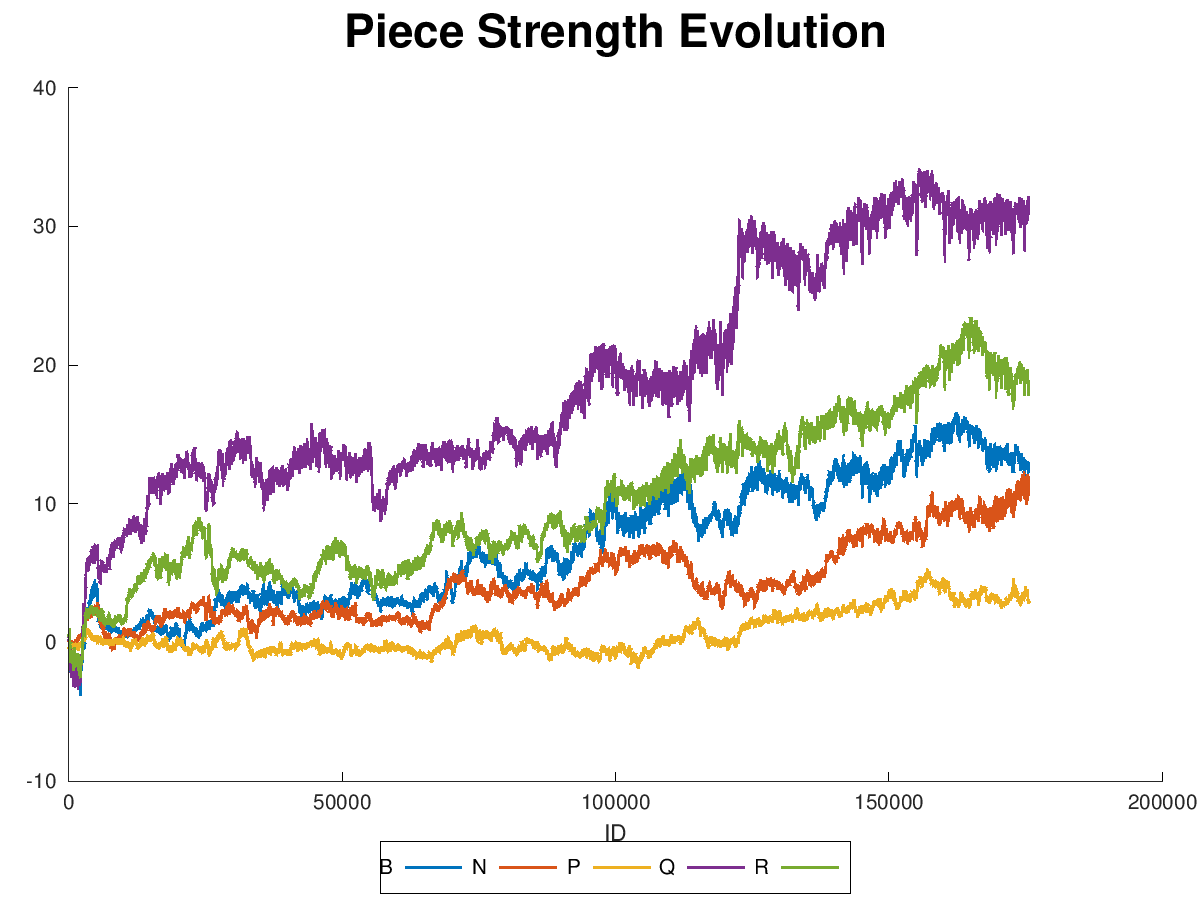
\includegraphics[width=\textwidth]{pawn-crash-strength-plot}
	\caption{The evolution of the value of pieces to the AIs. The small bump near ID~\#120,000 in the strength of a pawn that caused the Pawn Advancement Gene crash seen in Figure~\ref{pawn-crash}}\label{piece-value-plot}
\end{figure}

\subsubsection{Piece Strengths with the king}\label{piece-strength-with-king}

After assigning the king a strength entry in the Piece Strength Gene (see Section~\ref{piece-strength}), the other pieces retained their relative values, but the king evolved a very negative value. See Figure~\ref{piece-strength-with-king-plot}.
\begin{figure}[htb]
	\centering
	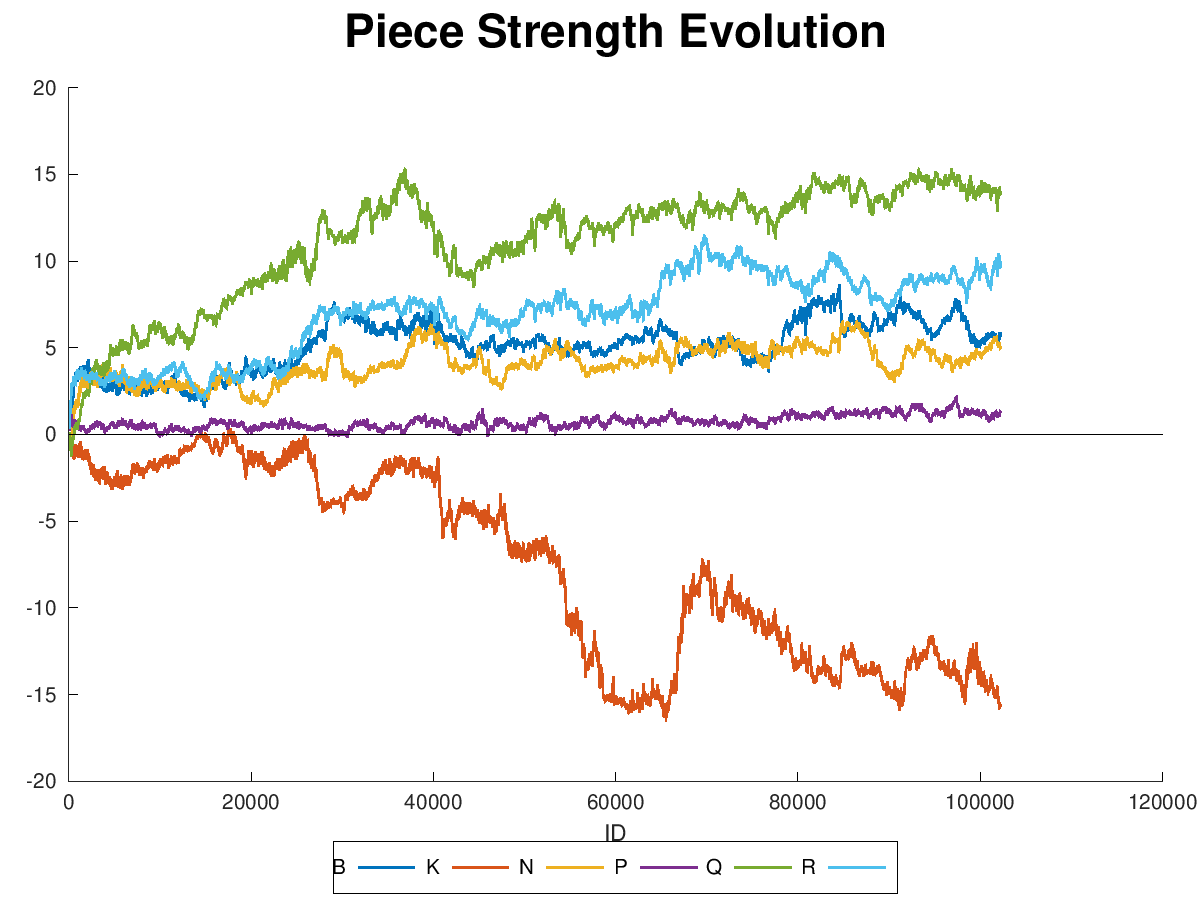
\includegraphics[width=\textwidth]{piece-strength-with-king-plot}
	\caption{The evolution of piece strengths after adding an entry for the king.}\label{piece-strength-with-king-plot}
\end{figure}

My current guess is that the king entry is affected by the Opponent Pieces Targeted  Gene and the Look-Ahead Gene---specifically the Capturing Speculation Constant. A large value for the Capturing Speculation Constant means that the board position that is actually evaluated has a smaller chance of having pieces threatened with capture. It is even less likely that the opponent's king is in check since this usually results in a reduced number of moves available, making recursion to the next move more likely. Thus, an evaluated board position with only the king in check is see as rather worthless unless offset by an attack on another piece that will probably result in capture. The king cannot be captured, so attacking it had better serve some other purpose. A similar evolution is seen in the Sphere of Influence Gene in that the King Target Factor is often negative.

This conclusion is corroborated by the King Target Bonus in the Opponent Pieces Targeted Gene (see Section~\ref{opponent-pieces-targeted}), which always has a negative or near-zero value that causes a preference for piece arrangements that attack more of the board away from the king.

\subsection{White has an advantage.}

Of the games ending in checkmate, white wins about 10\% more often than black. Figure~\ref{win-lose-plot} shows that the advantage is persistent through almost the whole of a long gene pool run. Wins by time are shared by black and white equally (see Figure~\ref{game-ending-plot}).
\begin{figure}[htb]
	\centering
	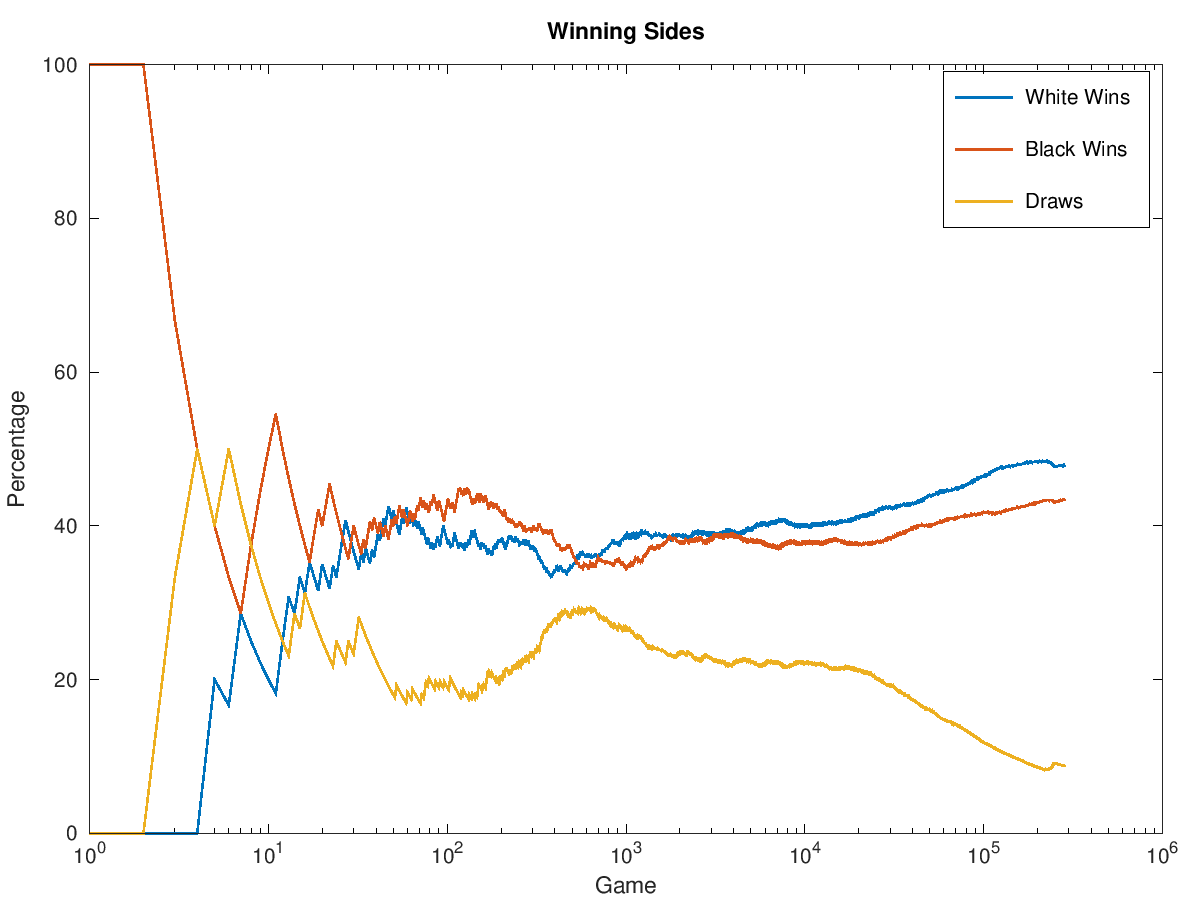
\includegraphics[width=\textwidth]{win-lose-plot}
	\caption{The percentage of games won by white, black, or neither over the course of a gene pool run. The advantage that white has over black seems persistent. Also, as the AIs evolve, the rate of draws decreases, presumably because they evolve a genome that can tell the difference between a good and bad position.}\label{win-lose-plot}
\end{figure}

\subsection{The Total Force Gene and the Pawn Advancement Gene typically dominate.}\label{total-force-and-pawn-result}

That the Total Force Gene dominates is fairly predictable. Highly skilled human players will usually resign after the loss of a minor (bishop or knight) piece without compensation.

The Pawn Advancement Gene usually gains higher priority first, probably because it is the simplest gene that makes an immediate difference in the game. Push the pawns forward both threatens the opponent's pieces with low-risk attacks and increases the chances of promotion.

\subsubsection{The Pawn Advancement Gene is a temporary substitute for a valid value of the pawn in the Piece Strength Gene.}\label{pawn-result}

Near the birth of the Genetic AI with ID~\#120,000, the Pawn Advancement Gene suddenly died off, with nearly all AIs in the gene pool deactivating the gene simultaneously (see Figure~\ref{pawn-crash}).
\begin{figure}[htb]
	\centering
	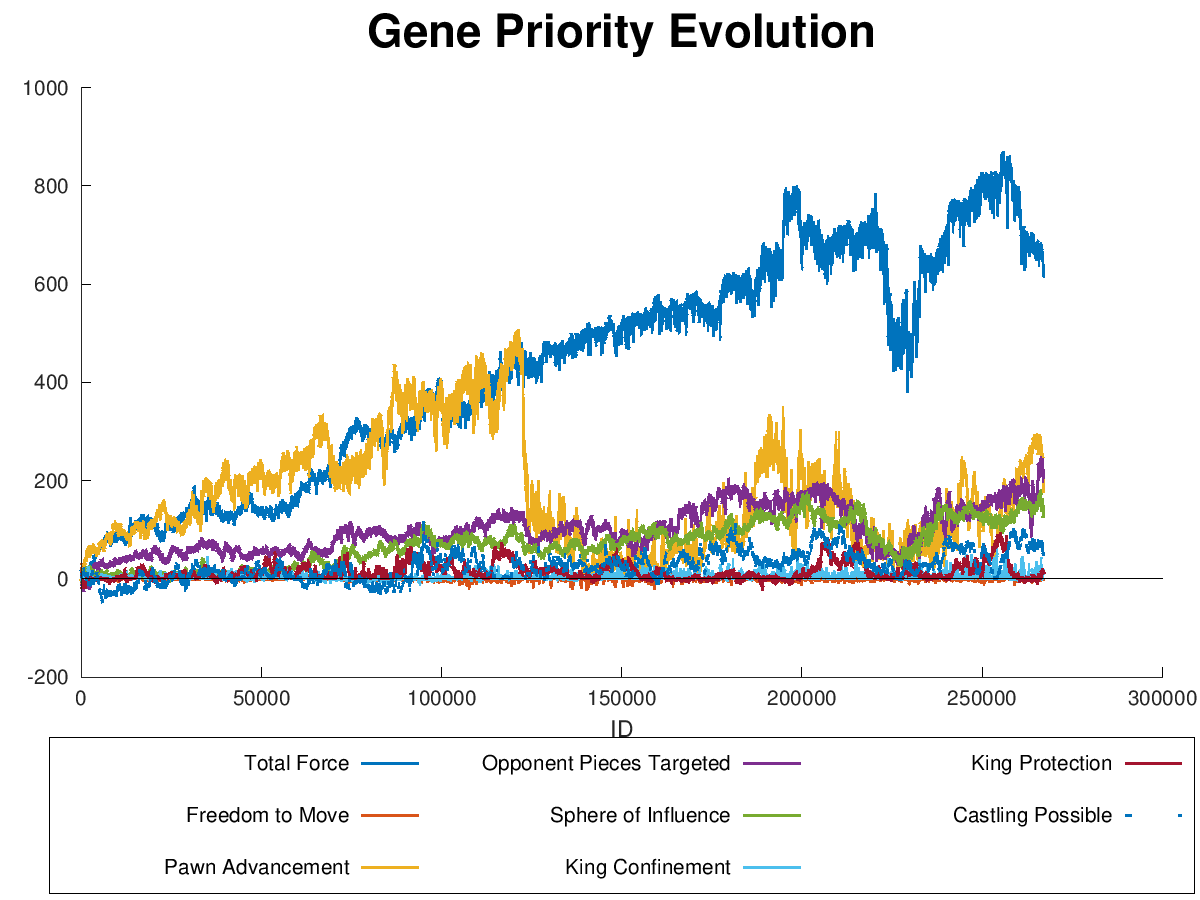
\includegraphics[width=0.7\textwidth]{pawn-advancement-crash}
	\caption{The sudden crash of the Pawn Advancement Gene}\label{pawn-crash}
\end{figure}

The only correlation with another gene near that time is in the Piece Strength Gene (see Figure~\ref{piece-value-plot}). The change is small, but in the comparison plot shown in Figure~\ref{pawn-crash}, one can see that the pawn strength has a small jump in value near ID~\#120,000. This is the first time that all of the AIs in the gene pools have strictly positive values for the pawn. Prior to this, the value of a pawn was zero on average. When mutations would push the pawn value higher, it would be weighted too much compared to other pieces, leading to losses and a lower value for the remaining population. It was only when the other pieces reached a large enough value that the pawn value could be properly weighted and sustained. Until this happened, the Pawn Advancement Gene evolved a large value in step with the Total Force Gene since pawns are not actually valueless in real games. Until the Piece Strength Gene transition occurred, the Pawn Advancement Gene served as a proxy for the value of a pawn that was more easily tuned in comparison with the Total Force Gene and Piece Strength Gene.

This pattern, in which a gene with a lower proper value or priority needs to wait for properly higher-priority genes to evolve high enough priorities before tuning their own priorities, is common and is discussed more the Section~\ref{lower-priority-waits}.

\subsection{The Queen is the most popular piece for promotion.}

Even when the Piece Strength Gene has not been tuned at all, the queen is the overwhelming favorite, followed by the rook, then bishop, and finally the knight. In human games, only the queen and knight are chosen since they have different move patterns. If you need at least a rook or bishop, you might as well take a queen since that piece provides both. Only the knight provides a viable alternative (usually to avoid a stalemate if the queen was chosen).

As an example, the following is a count of all promotions in a gene pool run after more than 300,000 games.
\begin{center}
\begin{tabular}{l r}
	Piece & Promotions \\
\toprule
	Bishop & 2232  \\
	Knight  &  1648 \\
	Rook    &  7215 \\
	Queen  & 146664 \\
\end{tabular}
\end{center}


\subsection{Threefold repetition is the most common stalemate.}

Most games with human players end in a draw when neither side can force an advantage. This happens when one side can block a crucial move (e.g., a pawn promotion) and the other side cannot remove this block. Since the blocking player does not have a reason to move, he can just repeat moves to maintain the block. This would lead to threefold repetition if most players did not verbally draw the game beforehand. Since these Genetic AI players don't offer or accept draws, they play out all the repetitions, resulting in what is seen in Figure~\ref{game-ending-plot}.

\subsection{The Look Ahead Gene is a late bloomer.}

The plot in Figure~\ref{game-ending-plot} shows the counts of how games end.
\begin{figure}[htb]
	\centering
	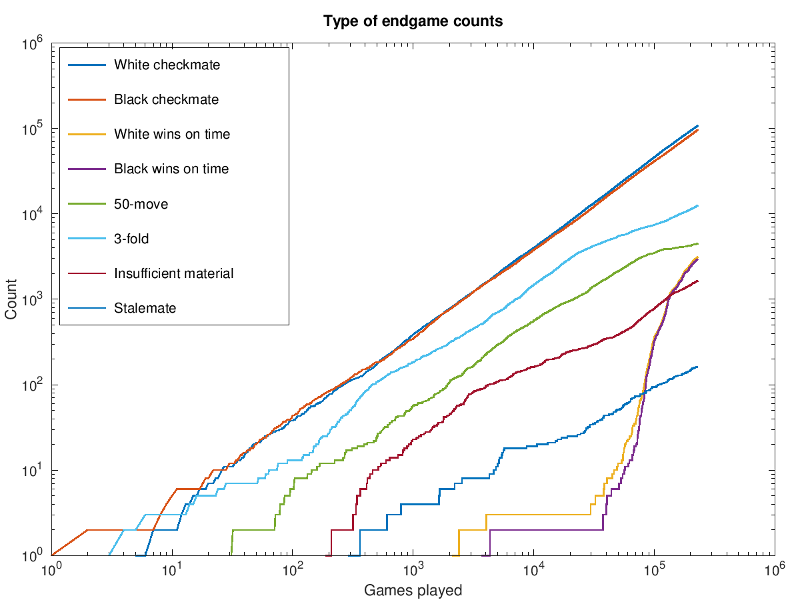
\includegraphics[width=\textwidth]{game-endings-log-plot}
	\caption{A log-log scale of the percentage of games with various endings. Note that the time forfeits don't get going until about 30,000 games in.}\label{game-ending-plot}
\end{figure}
It seems that the Look Ahead Gene does not experience significant evolutionary pressure until the board-scoring genes have been tuned to a semi-decent state. My hypothesis is that if the board-scoring function is not able to tell a good position from bad, then looking ahead only increases the risk of losing by time forfeiture with no benefit. However, when the board-scoring genes are in a decent state, the increase in look ahead is very quick. This leads to a rapid increase in the rate of deaths by running out of time, but apparently this is worth the risk as those who are more conservative with their time lose to those who see farther ahead.

\subsection{The Sphere of Influence Gene typically counts legal moves as having lower value than other moves.}

This was unexpected. I thought that the legal moves would count more since they present a greater threat to the opponent. You cannot capture your opponent's Queen if your own King is in check. Perhaps Genetic\_AIs find this gene more useful as a forward-looking view of the game. Or, the Opponent Pieces Targeted Gene relieves this gene of having to consider legal moves (much the same as how the Pawn value in the Piece Strength Gene and the priority of the Pawn Advancement Gene interact (Section~\ref{pawn-result})).

\subsection{Genes with properly lower priorities have to wait for higher priority genes to evolve their higher priority before evolving themselves.}\label{lower-priority-waits}

Some genes are more important than others. The Total Force Gene dominates because it is nearly always more difficult to win when behind in pieces. So, if another gene evolves too high a priority, it hinders game play and will soon be killed off. This means that, because the rate of evolution is the same for all gene priorities, that genes with a lower proper priority\footnote{By proper priority, I mean the as yet unknown relative priority compared with other genes that leads to winning game play. The proper priorities are what this program should be evolving towards.} need to wait for those genes with higher proper priority to evolve a large enough value. Before then, it is too likely for a random mutation to push a lower priority too high and get a gene killed off.

The same goes for the Piece Strength Gene with respect to the value of each type of piece. Note in Figure~\ref{piece-value-plot} that the values rise and fall with each other.

\section{Programming Quirks}

Since this software is still in heavy development, the following sections are likely to change. As such, here is a summary of aspects of the code that might seem weird upon first---and possibly every other---reading. Specifically, if this is modern \cpp{}, why are there pointers everywhere?

Though the operators \code{new} and \code{delete} appear nowhere in the code and smart pointers are used, raw pointers appear everywhere in the code. The driving reason for using pointers is polymorphic storage. Classes representing moves are derived from a \code{Move} so that they can override various legality and side-effect methods. Storing different types of moves requires storing \code{Move*}s. The same goes for \code{Gene} storage in the \code{Genome} class.

Originally, instances of the \code{Board} class contained an array of \code{std::shared\_ptr}s so that copying a board (for when computer players needed to think ahead) did not present difficulties in managing the piece resources (namely, when to call \code{delete}). While easy to code, the bookkeeping required by shared pointer copying slowed down the speed of the AIs traversal of the game tree. Then, each type and color of piece was stored as a static instance in the \code{Board} class and pointers to these instances are used as markers for board positions. While this does mean that \code{Piece} classes are treated like singletons (or, rather, doubletons, since there are black and white instances), this was simpler and faster. The pieces in this code do not have any modifiable internal state after creation, so any two white pawn--even ones taken from different boards--should be completely indistinguishable. In the most recent version, every piece is simply an unsigned integer where individual bits represent the color and type of a piece. This is the simplest and fastest way to represent an entity with no state other than its identity. The integer representation is used to access arrays of pointers to \code{Move}s.

If a function or method returns a pointer, the caller of that function is not responsible for deleting the data pointed to by the pointer (and, in fact, should not). Most public methods and functions take reference arguments to prevent problems with null pointers. Where functions do take pointer arguments (such as \code{Board::print\_game\_record()} for the player instances), that argument is optional parameter that can take a \code{nullptr} to indicate no data.


\begin{thebibliography}{99}

\bibitem{evolved-antenna}
G.S. Hornby, A. Globus, D.S. Linden, J.D. Lohn, ``Automated Antenna Design with Evolutionary Algorithms.'' AIAA

\bibitem{evolved-stellarator}
W.H. Miner, Jr., P.M. Valanju, S.P. Hirshman, A. Brooks, N. Pomphrey, ``Use of a genetic algorithm for compact stellarator coil design.'' IAEA Nuclear Fusion, Vol. 41, No. 9. 1185--1195

\bibitem{log-norm-wiki}
\url{https://en.wikipedia.org/wiki/Log-normal\_distribution}

\bibitem{log-norm-chess-se}
\url{https://chess.stackexchange.com/a/4899/5819}

\bibitem{quiescence-ref}
\url{https://www.chessprogramming.org/Quiescence_Search}

\bibitem{fen-notation}
\url{http://www.thechessdrum.net/PGN_Reference.txt} Section~16.1

\bibitem{turing-chess}
Turing, Alan M., ``Digital Computers Applied to Games.'' Faster Than Thought. B. V. Bowden. London: Sir Isaac Pitman \& Sons, Ltd., 1953, pg. 286--297. Print.

\bibitem{monte-carlo}
\url{https://en.wikipedia.org/wiki/Monte_Carlo_tree_search}

\bibitem{recombination-wiki}
\url{https://en.wikipedia.org/wiki/Genetic_recombination}

\bibitem{evolution-strategy-wiki}
\url{https://en.wikipedia.org/wiki/Evolution_strategy}

\bibitem{evolution-strategy-glossary}
\url{http://ls11-www.cs.tu-dortmund.de/~beyer/EA-glossary/node41.html}

\end{thebibliography}

\end{document}
